\documentclass[12pt]{report}
% PACKAGES
\usepackage[a4paper,bindingoffset=0in,
            left=1in,right=1in,top=1in,bottom=1.5in,
            footskip=.5in]{geometry}
\usepackage{lastpage}
\usepackage[ddmmyyyy]{datetime}
\usepackage{amsmath}    % need for subequations
\usepackage{graphicx}   % need for figures
\usepackage{verbatim}   % useful for program listings
\usepackage{color}      % use if color is used in text
\usepackage{subfigure}  % use for side-by-side figures
\usepackage{hyperref}   % use for hypertext links, including those to external documents and URLs
\usepackage{fancyhdr}   % for image in header
\usepackage[outline]{contour} %contorno
\usepackage{float}
\restylefloat{table}
\usepackage[table,xcdraw]{xcolor}
\usepackage{screenplay-pkg}
\usepackage{eso-pic}
\usepackage{pst-text}
\usepackage{transparent} % TRASPARENZA
\usepackage{efbox} % PER ETICHETTA
\usepackage{tabularx}
\usepackage{longtable}
\usepackage[autostyle]{csquotes}

\expandafter\def\expandafter\UrlBreaks\expandafter{\UrlBreaks%  save the current one
  \do\*\do\-\do\~\do\'\do\"\do\-}

\usepackage{titlesec}
\newcommand{\sectionbreak}{\clearpage}

\newlength{\mydimen}
\setlength{\mydimen}{10mm}

\setlength{\parskip}{6pt}
\setlength{\parindent}{0pt}

\hypersetup{
    colorlinks=false,
  	pdfborder={0 0 0} % border style will be underline of width 1pt
}


%%%%%%%%%%%%%%%%%%%%%%%%%%%%%%%%%%%%%%%%%%%%%%%%%%%%%%%%%%%%%%%%%%%%%%%%%%%%%%%%%%%%%%%%%%%%%%%%%%%%%%%%%%

% HEADER and FOOTER
\pagestyle{fancy}{
  \lhead{
\includegraphics[width=5cm]{../../Logos/logoUnimi_small}}
  \rhead{
\includegraphics[width=5cm]{../../Logos/logoPong_small}}
  \lfoot{Last updated: \today}
  \cfoot{ }
  \rfoot{Page \thepage\ of \pageref{LastPage}}
}

\patchcmd{\chapter}{\thispagestyle{plain}}{\thispagestyle{fancy}}{}{}

\begin{document}

\thispagestyle{empty}{}

% logoTeam
\begin{center}
  \begin{figure}[H]
    \centering
    \vspace*{30pt}
    
\includegraphics[width=12cm]{../../Logos/logoTeam_big}
  \end{figure}

  \vspace{50pt}
  
  \scalebox{1.5}{\contour{black}{\textbf{ \textcolor{white}{\huge Sophie's Flying Castle}}}}
  
  \scalebox{1.5}{\contour{black}{\textbf{ \textcolor{white}{\Large \textbf{Dungeons \& Djinns}}}}}

  \scalebox{1.5}{\contour{black}{\textbf{ \textcolor{white}{\large \textbf{Level 3. In enemy territory}}}}}
  
  \vspace{20pt}

  \scalebox{1.5}{\contour{black}{ \textbf{ \textcolor{white}{\large \textbf{\textit{Game and Level Design 2018/19}}}}}}
\end{center}

\AddToShipoutPictureBG*{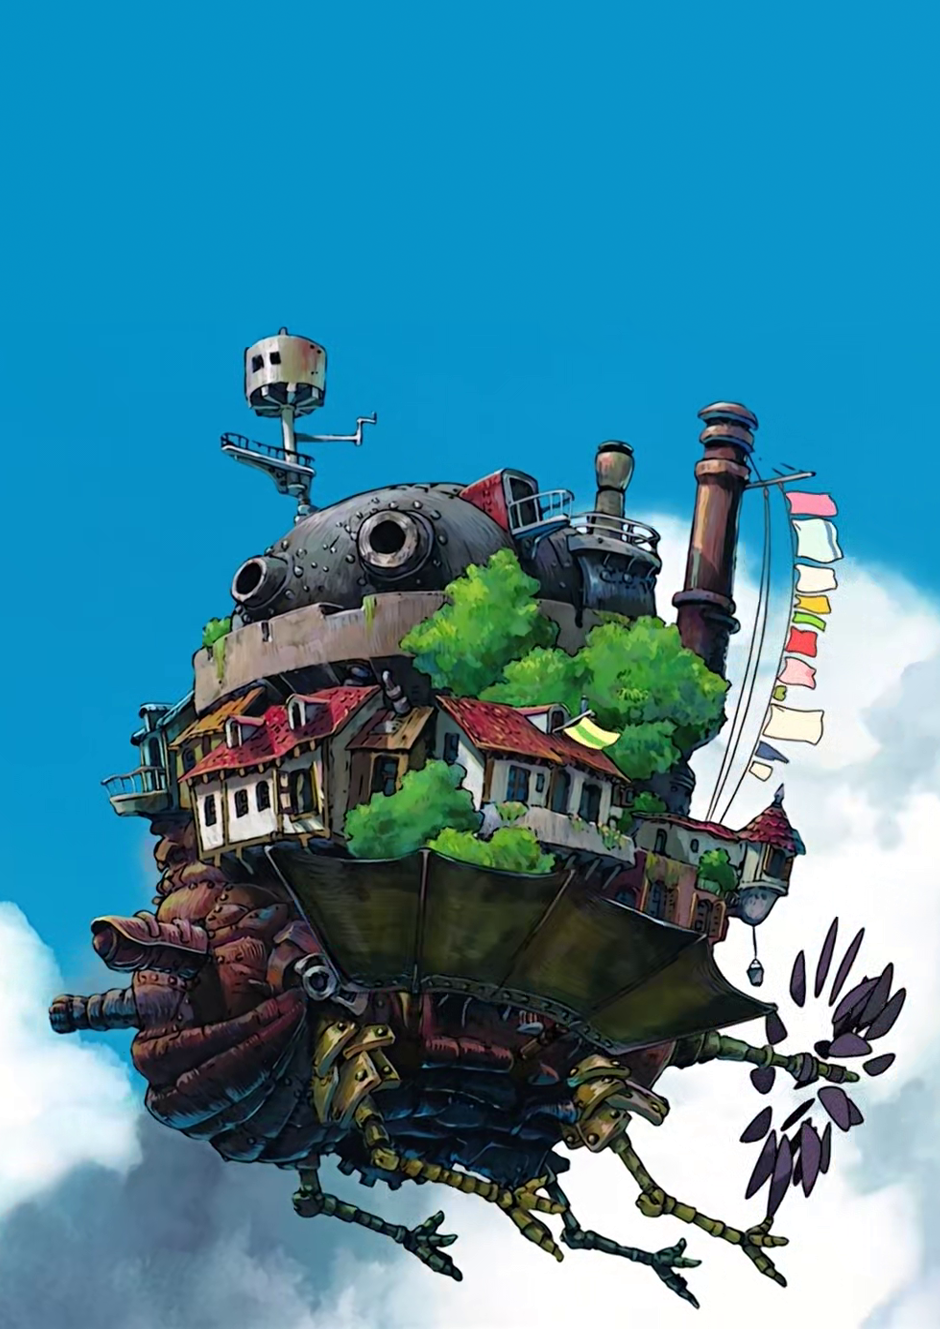
\includegraphics[width=\paperwidth,height=\paperheight,keepaspectratio]{../../Logos/flyingCastle_cover}}

\vspace{170pt}
\setlength{\fboxrule}{1pt}

\begin{table}[H]
  \centering
  \efbox[backgroundcolor=white]{	
	\begin{tabular}{lcr}
    \textbf{Francesco Periti} & \underline{\href{mailto:francesco.periti@studenti.unimi.it}{francesco.periti@studenti.unimi.it}} & 930650 \\
    \textbf{Francesco Principe} & \underline{\href{mailto:francesco.principe@studenti.unimi.it}{francesco.principe@studenti.unimi.it}} & 937622 \\
    \textbf{Davide Valentini} & \underline{\href{mailto:davide.valentini1@studenti.unimi.it}{davide.valentini1@studenti.unimi.it}} & 939054 \\
    \textbf{Elena Coperchini} & \underline{\href{mailto:elena.coperchini@gmail.com}{elena.coperchini@gmail.com}} & \\
	\end{tabular}}
\end{table}

\vspace*{20pt}

\scalebox{1.5}{\large \textbf{Level 3. In enemy territory}}

\scalebox{1.5}{\textbf{Map: Dynamia}}

\begin{figure}[H]
  \centering
  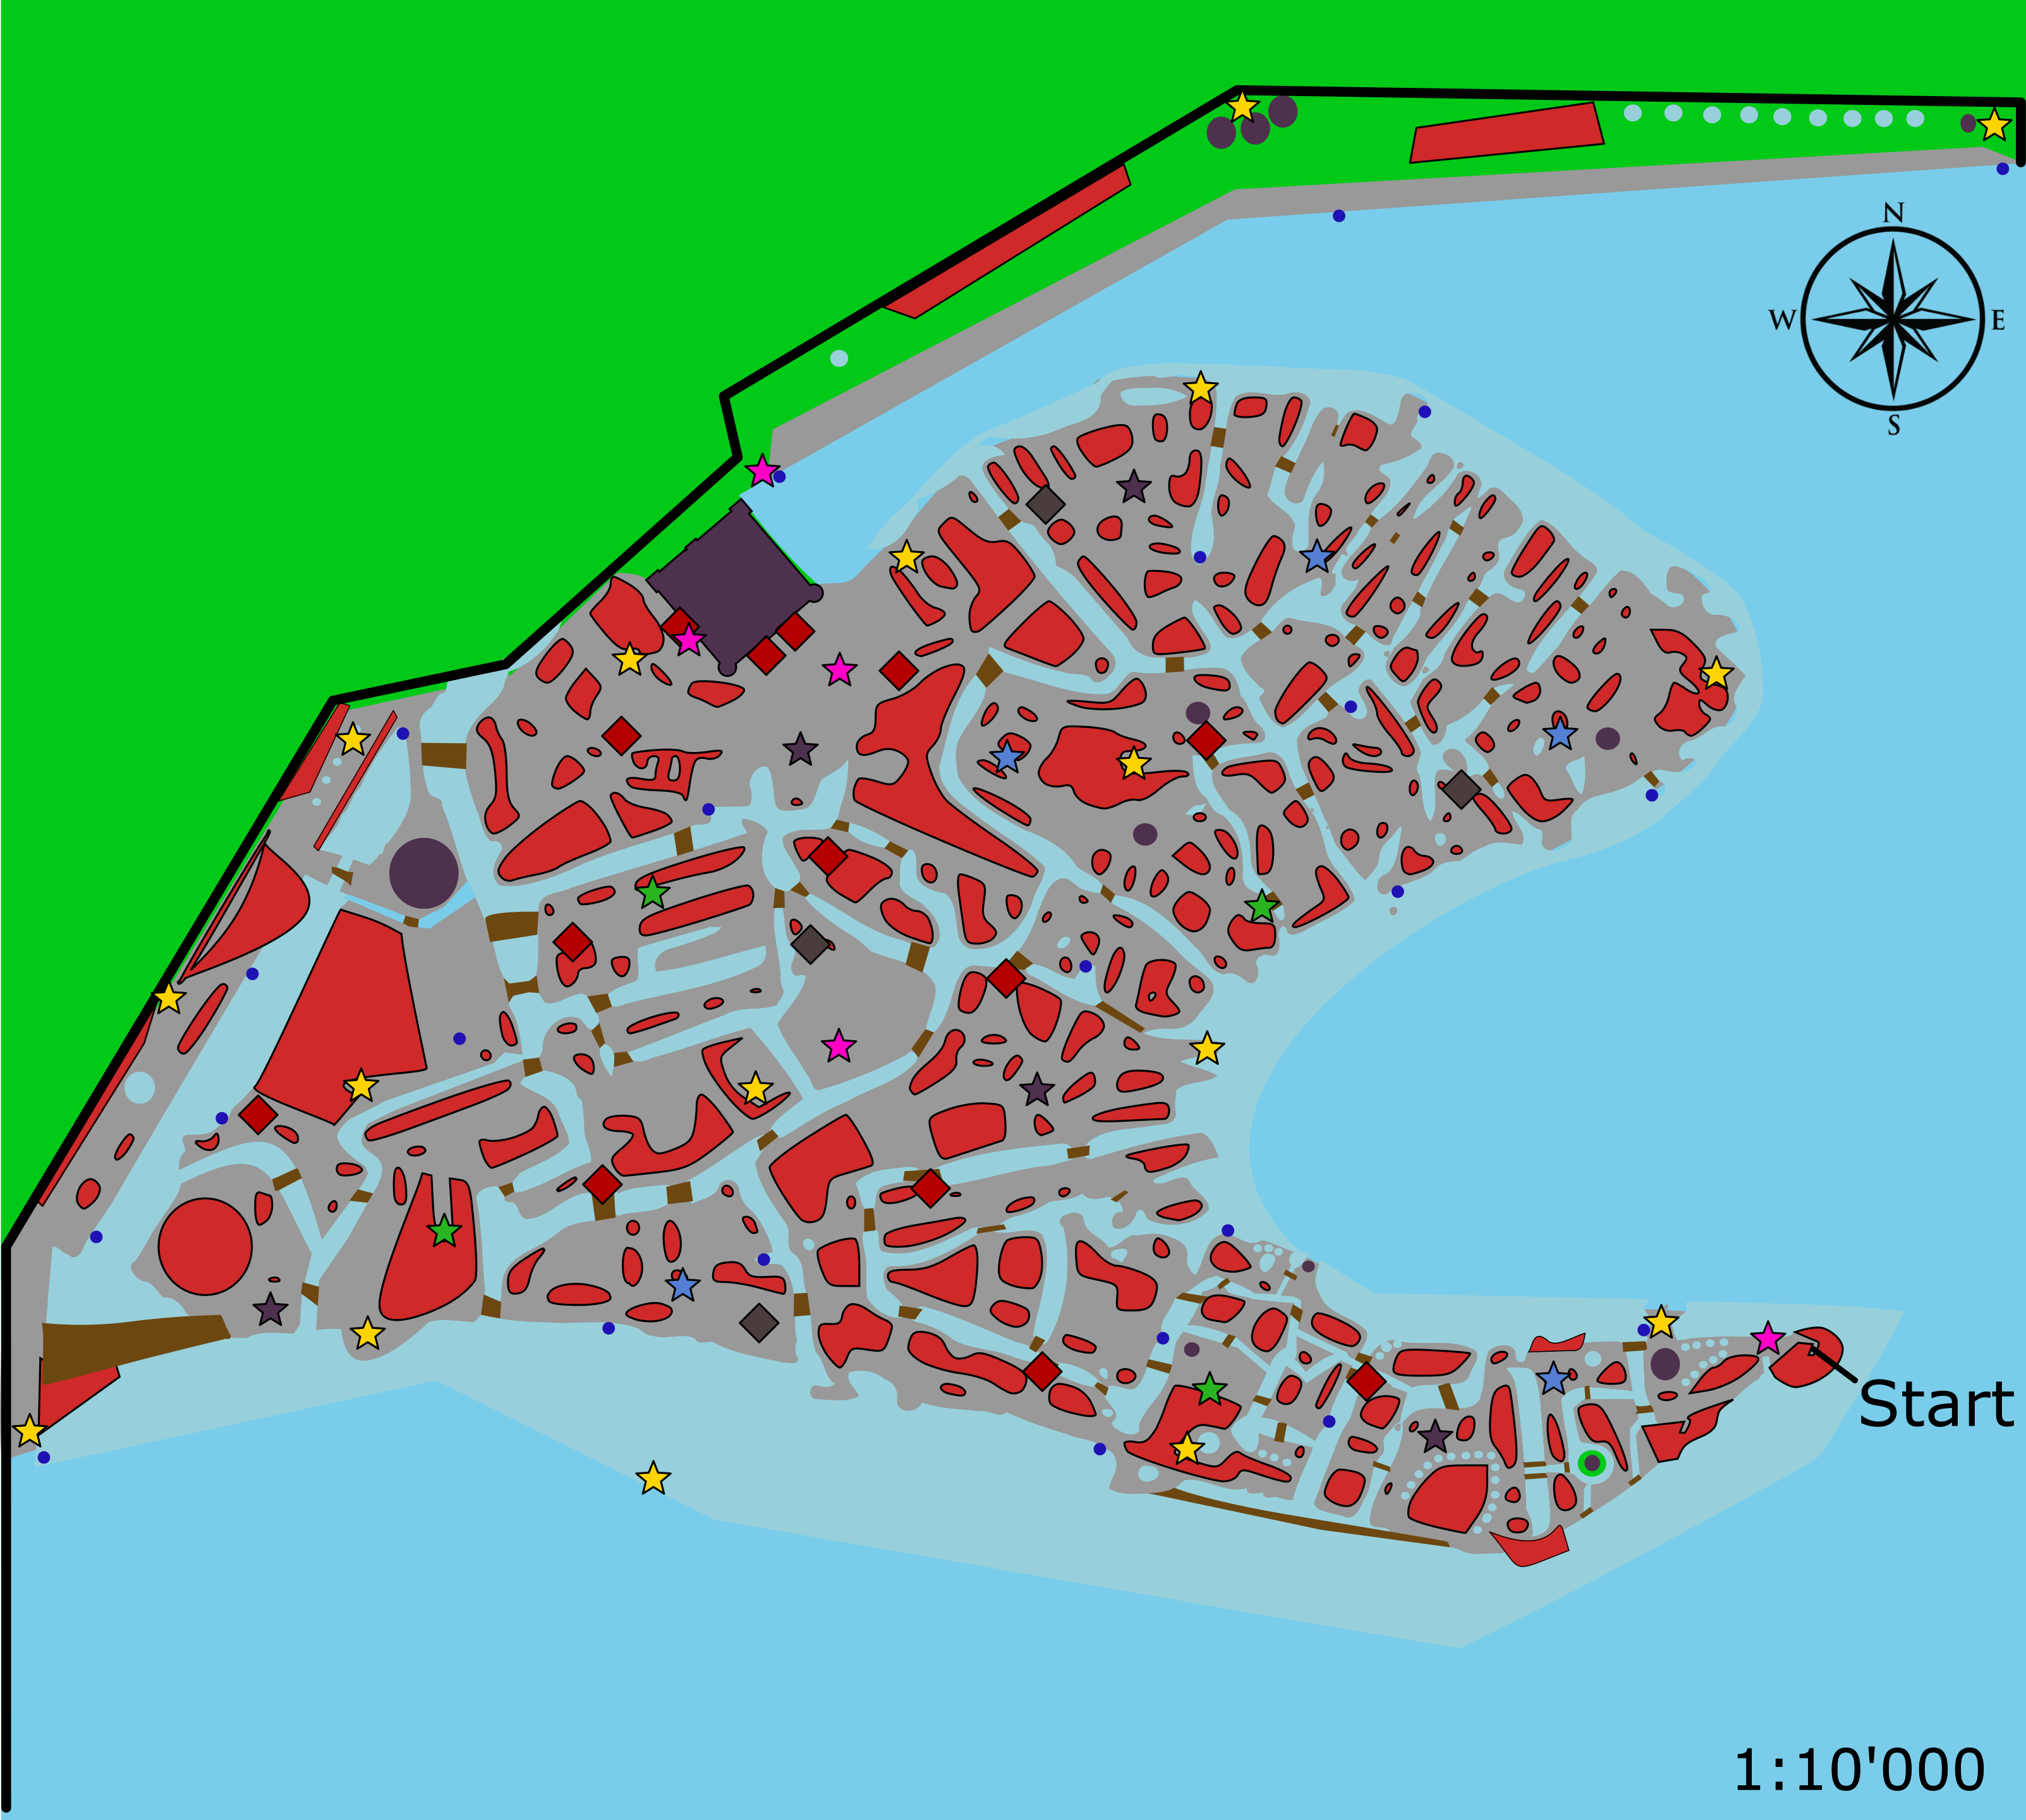
\includegraphics[width=\textwidth]{Images/Maps/dynamiaCover}
\end{figure}


\section*{Revision History}
\begin{table}[H]
\centering
  \begin{tabularx}{\textwidth}{|l|l|X|}
\hline
\cellcolor{lightgray}\textbf{Who} & \cellcolor{lightgray}\textbf{When} & \cellcolor{lightgray}\textbf{What} \\ \hline
Francesco Periti & 02/11/2018 & Created this document \\ \hline
Francesco Periti & 03/11/2018 & Added some conventions to directories structure \\ \hline
Davide Valentini & 03/11/2018 & Added e-mail references \\ \hline
Francesco Principe & 04/11/2018 & Added some conventions to file naming \\ \hline
Davide Valentini & 04/11/2018 & Added software list \\ \hline
Francesco Principe & 05/11/2018 & Global revision \\ \hline
Davide Valentini & 06/11/2018 & Added file access rules \\ \hline
Francesco Periti & 06/11/2018 & Added repository structure rules \\ \hline
Davide Valentini & 07/11/2018 & Added owners and editors rules \\ \hline
Francesco Periti & 08/11/2018 & Global revision \\ \hline
Francesco Periti & 18/11/2018 & Added game title \\ \hline
Francesco Periti & 21/11/2018 & Global revision \\ \hline
Francesco Principe & 26/11/2018 & Added work directories structure \\ \hline
Francesco Principe & 26/11/2018 & Added some permissions \\ \hline
Davide Valentini & 26/11/2018 & Remove audio, video, 3d models \\ \hline
Davide Valentini & 26/11/2018 & Added some conventions \\ \hline
Francesco Principe & 26/11/2018 & Added file naming conventions section\\ \hline

Davide Valentini & 26/11/2018 & Added some directory to the structure\\ \hline
Francesco Periti & 28/11/2018 & Added conventions for new directories\\ \hline
Francesco Principe & 28/11/2018 & Editet conventions for new directories\\ \hline
Davide Valentini & 29/11/2018 & Added permissions for new directories\\ \hline
Francesco Principe & 30/11/2018 & Added some directory to the structure\\ \hline
Francesco Principe & 1/12/2018 & Added some directory to the structure\\ \hline
Davide Valentini & 4/12/2018 & Added file naming conventions\\ \hline
Davide Valentini & 5/12/2018 & Added conventions for new directories\\ \hline
Davide Valentini & 6/12/2018 & Edited directories structure and relative conventions\\ \hline
Francesco Periti & 6/12/2018 & Added some directory to the structure\\ \hline
Francesco Periti & 6/12/2018 & Added conventions for new directories\\ \hline
Francesco Principe & 10/12/2018 &  Added rows for table in data type and format\\ \hline
Francesco Principe & 10/12/2018 & Added file naming conventions\\ \hline
Francesco Periti & 10/12/2018 & Added website section\\ \hline
Francesco Periti & 11/12/2018 & Global revision\\ \hline
Francesco Periti & 27/12/2018 & Added some directory to the structure\\ \hline
Davide Valentini & 30/12/2018 & Added conventions for new directories\\ \hline
Francesco Principe & 3/01/2019 & Global revision\\ \hline

\end{tabularx}
\end{table}


\tableofcontents

\part{Game overview}

\chapter{Game Skills}

\section{Skills Chart}
%ho salvato la tabella da inserire in formato tgn. Quando siamo insieme, aprima il sito magico e la generiamo come crediamo

\section{Skills}
During the game the player can use many skills while impersonating Sophie.

The following table shows how the skills are distributed throughout the game.

\begin{longtable}[H]{|p{1.7cm}|p{1.7cm}|p{1.7cm}|p{1.7cm}|p{1.7cm}|p{1.7cm}|p{1.7cm}|p{1.7cm}|}
  \hline
\cellcolor[HTML]{656565}{\color[HTML]{FFFFFF} \textbf{Skill}} & \cellcolor[HTML]{C0C0C0}{\color[HTML]{330001} \textbf{First steps}} & \cellcolor[HTML]{C0C0C0}{\color[HTML]{330001} \textbf{Where is Howl?}} & \cellcolor[HTML]{C0C0C0}{\color[HTML]{330001} \textbf{In enemy territory}} & \cellcolor[HTML]{C0C0C0}{\color[HTML]{330001} \textbf{Nasty surprise(s)}} & \cellcolor[HTML]{C0C0C0}{\color[HTML]{330001} \textbf{The djiin of the desert}} & \cellcolor[HTML]{C0C0C0}{\color[HTML]{330001} \textbf{The spirts realm}} & \cellcolor[HTML]{C0C0C0}{\color[HTML]{330001} \textbf{Fire and secrets}} \\ \hline
\textbf{Magic Door} & X & X & X & X &  & X &  \\ \hline
\textbf{Sewing} & X & O & O & O & O & O & O \\ \hline
\textbf{Talk to objects} & X & X & X & O & O & X & X \\ \hline
\textbf{Magic lantern} &  & O & X & X &  & X & X \\ \hline
\textbf{Multi-option dialogue} &  & X & X & X & X & X &  \\ \hline
%\textbf{Lantern trasformation} &  &  & X &  & X & X &  \\ \hline
\textbf{Pilot the castle} &  &  &  &  & X &  &X  \\ \hline
%\textbf{Sailing} &  &  & X &  &  & X &  \\ \hline
\textbf{Metamor-phosis} &  &  &  &  &  &  & X \\ \hline
\end{longtable}

\textbf{X}: the skill is required \\
\textbf{O}: the skill may be used, but it is not required

\begin{itemize}
\item \textbf{Magic door}: Sophie uses the flying castle's magic door to rapidly move through the levels.
\item \textbf{Sewing}: Sophie can sew magic hats with the magic needle in the flying castle. Each hat requires some crafting materials.
\item \textbf{Talk to objects}: Sophie uses this skill to have dialogues with objects. Just some objects can interact with her. They give her information, tips, rewards or other.
\item \textbf{Magic lantern}: Sophie uses the magic lantern to control Calcifer during a fight.
\item \textbf{Multi-option dialogue}: during a dialogue Sophie has some options to choose from.
%\item \textbf{Lantern transformation}: during the game Calcifer can use scraps, objects or other to transform temporarily his lantern in some useful machine. %Sophie can control this skills. Just in some part of the game she has to use.
\item \textbf{Pilot the castle}: Sophie pilots the flying castle.
%\item \textbf{Sailing}: Sophie use this skill to sail a boat.
\item \textbf{Metamorphosis}: Sophie can allow Calcifer to turn into a powerful demon. This skill is used only in the last level where the player will control Calcifer to defeat Mizar.
\end{itemize}

\subsection{Magic lantern skills}
There are several combinations of attack that Calcifer can do in the game, they are not essential to finish the game or overpass levels. They just increase in some way the value attack:\\
TODO
\subsubsection{Pugno di fuoco}
\begin{table}[H]
  \centering
\begin{tabular}{|
>{\columncolor[HTML]{C0C0C0}}l |l|}
\hline
\textbf{Name} & Pugno di fuoco \\ \hline
\textbf{Saving Throw} &  \\ \hline
\textbf{Description} &  \\ \hline
\textbf{Range} &  \\ \hline
\textbf{Duration} &  \\ \hline
\textbf{Description} &  \\ \hline
\end{tabular}
\end{table}
\subsubsection{Calcio volante multiplo}
\begin{table}[H]
  \centering
\begin{tabular}{|
>{\columncolor[HTML]{C0C0C0}}l |l|}
\hline
\textbf{Name} & Pugno di fuoco \\ \hline
\textbf{Saving Throw} &  \\ \hline
\textbf{Description} &  \\ \hline
\textbf{Range} &  \\ \hline
\textbf{Duration} &  \\ \hline
\textbf{Description} &  \\ \hline
\end{tabular}
\end{table}




\chapter{Game Skills}

\section{Skills Chart}
%ho salvato la tabella da inserire in formato tgn. Quando siamo insieme, aprima il sito magico e la generiamo come crediamo

\section{Skills}
During the game the player can use many skills while impersonating Sophie.

The following table shows how the skills are distributed throughout the game.

\begin{longtable}[H]{|p{1.7cm}|p{1.7cm}|p{1.7cm}|p{1.7cm}|p{1.7cm}|p{1.7cm}|p{1.7cm}|p{1.7cm}|}
  \hline
\cellcolor[HTML]{656565}{\color[HTML]{FFFFFF} \textbf{Skill}} & \cellcolor[HTML]{C0C0C0}{\color[HTML]{330001} \textbf{First steps}} & \cellcolor[HTML]{C0C0C0}{\color[HTML]{330001} \textbf{Where is Howl?}} & \cellcolor[HTML]{C0C0C0}{\color[HTML]{330001} \textbf{In enemy territory}} & \cellcolor[HTML]{C0C0C0}{\color[HTML]{330001} \textbf{Nasty surprise(s)}} & \cellcolor[HTML]{C0C0C0}{\color[HTML]{330001} \textbf{The djiin of the desert}} & \cellcolor[HTML]{C0C0C0}{\color[HTML]{330001} \textbf{The spirts realm}} & \cellcolor[HTML]{C0C0C0}{\color[HTML]{330001} \textbf{Fire and secrets}} \\ \hline
\textbf{Magic Door} & X & X & X & X &  & X &  \\ \hline
\textbf{Sewing} & X & O & O & O & O & O & O \\ \hline
\textbf{Talk to objects} & X & X & X & O & O & X & X \\ \hline
\textbf{Magic lantern} &  & O & X & X &  & X & X \\ \hline
\textbf{Multi-option dialogue} &  & X & X & X & X & X &  \\ \hline
%\textbf{Lantern trasformation} &  &  & X &  & X & X &  \\ \hline
\textbf{Pilot the castle} &  &  &  &  & X &  &X  \\ \hline
%\textbf{Sailing} &  &  & X &  &  & X &  \\ \hline
\textbf{Metamor-phosis} &  &  &  &  &  &  & X \\ \hline
\end{longtable}

\textbf{X}: the skill is required \\
\textbf{O}: the skill may be used, but it is not required

\begin{itemize}
\item \textbf{Magic door}: Sophie uses the flying castle's magic door to rapidly move through the levels.
\item \textbf{Sewing}: Sophie can sew magic hats with the magic needle in the flying castle. Each hat requires some crafting materials.
\item \textbf{Talk to objects}: Sophie uses this skill to have dialogues with objects. Just some objects can interact with her. They give her information, tips, rewards or other.
\item \textbf{Magic lantern}: Sophie uses the magic lantern to control Calcifer during a fight.
\item \textbf{Multi-option dialogue}: during a dialogue Sophie has some options to choose from.
%\item \textbf{Lantern transformation}: during the game Calcifer can use scraps, objects or other to transform temporarily his lantern in some useful machine. %Sophie can control this skills. Just in some part of the game she has to use.
\item \textbf{Pilot the castle}: Sophie pilots the flying castle.
%\item \textbf{Sailing}: Sophie use this skill to sail a boat.
\item \textbf{Metamorphosis}: Sophie can allow Calcifer to turn into a powerful demon. This skill is used only in the last level where the player will control Calcifer to defeat Mizar.
\end{itemize}

\subsection{Magic lantern skills}
There are several combinations of attack that Calcifer can do in the game, they are not essential to finish the game or overpass levels. They just increase in some way the value attack:\\
TODO
\subsubsection{Pugno di fuoco}
\begin{table}[H]
  \centering
\begin{tabular}{|
>{\columncolor[HTML]{C0C0C0}}l |l|}
\hline
\textbf{Name} & Pugno di fuoco \\ \hline
\textbf{Saving Throw} &  \\ \hline
\textbf{Description} &  \\ \hline
\textbf{Range} &  \\ \hline
\textbf{Duration} &  \\ \hline
\textbf{Description} &  \\ \hline
\end{tabular}
\end{table}
\subsubsection{Calcio volante multiplo}
\begin{table}[H]
  \centering
\begin{tabular}{|
>{\columncolor[HTML]{C0C0C0}}l |l|}
\hline
\textbf{Name} & Pugno di fuoco \\ \hline
\textbf{Saving Throw} &  \\ \hline
\textbf{Description} &  \\ \hline
\textbf{Range} &  \\ \hline
\textbf{Duration} &  \\ \hline
\textbf{Description} &  \\ \hline
\end{tabular}
\end{table}




\chapter{Game Skills}

\section{Skills Chart}
%ho salvato la tabella da inserire in formato tgn. Quando siamo insieme, aprima il sito magico e la generiamo come crediamo

\section{Skills}
During the game the player can use many skills while impersonating Sophie.

The following table shows how the skills are distributed throughout the game.

\begin{longtable}[H]{|p{1.7cm}|p{1.7cm}|p{1.7cm}|p{1.7cm}|p{1.7cm}|p{1.7cm}|p{1.7cm}|p{1.7cm}|}
  \hline
\cellcolor[HTML]{656565}{\color[HTML]{FFFFFF} \textbf{Skill}} & \cellcolor[HTML]{C0C0C0}{\color[HTML]{330001} \textbf{First steps}} & \cellcolor[HTML]{C0C0C0}{\color[HTML]{330001} \textbf{Where is Howl?}} & \cellcolor[HTML]{C0C0C0}{\color[HTML]{330001} \textbf{In enemy territory}} & \cellcolor[HTML]{C0C0C0}{\color[HTML]{330001} \textbf{Nasty surprise(s)}} & \cellcolor[HTML]{C0C0C0}{\color[HTML]{330001} \textbf{The djiin of the desert}} & \cellcolor[HTML]{C0C0C0}{\color[HTML]{330001} \textbf{The spirts realm}} & \cellcolor[HTML]{C0C0C0}{\color[HTML]{330001} \textbf{Fire and secrets}} \\ \hline
\textbf{Magic Door} & X & X & X & X &  & X &  \\ \hline
\textbf{Sewing} & X & O & O & O & O & O & O \\ \hline
\textbf{Talk to objects} & X & X & X & O & O & X & X \\ \hline
\textbf{Magic lantern} &  & O & X & X &  & X & X \\ \hline
\textbf{Multi-option dialogue} &  & X & X & X & X & X &  \\ \hline
%\textbf{Lantern trasformation} &  &  & X &  & X & X &  \\ \hline
\textbf{Pilot the castle} &  &  &  &  & X &  &X  \\ \hline
%\textbf{Sailing} &  &  & X &  &  & X &  \\ \hline
\textbf{Metamor-phosis} &  &  &  &  &  &  & X \\ \hline
\end{longtable}

\textbf{X}: the skill is required \\
\textbf{O}: the skill may be used, but it is not required

\begin{itemize}
\item \textbf{Magic door}: Sophie uses the flying castle's magic door to rapidly move through the levels.
\item \textbf{Sewing}: Sophie can sew magic hats with the magic needle in the flying castle. Each hat requires some crafting materials.
\item \textbf{Talk to objects}: Sophie uses this skill to have dialogues with objects. Just some objects can interact with her. They give her information, tips, rewards or other.
\item \textbf{Magic lantern}: Sophie uses the magic lantern to control Calcifer during a fight.
\item \textbf{Multi-option dialogue}: during a dialogue Sophie has some options to choose from.
%\item \textbf{Lantern transformation}: during the game Calcifer can use scraps, objects or other to transform temporarily his lantern in some useful machine. %Sophie can control this skills. Just in some part of the game she has to use.
\item \textbf{Pilot the castle}: Sophie pilots the flying castle.
%\item \textbf{Sailing}: Sophie use this skill to sail a boat.
\item \textbf{Metamorphosis}: Sophie can allow Calcifer to turn into a powerful demon. This skill is used only in the last level where the player will control Calcifer to defeat Mizar.
\end{itemize}

\subsection{Magic lantern skills}
There are several combinations of attack that Calcifer can do in the game, they are not essential to finish the game or overpass levels. They just increase in some way the value attack:\\
TODO
\subsubsection{Pugno di fuoco}
\begin{table}[H]
  \centering
\begin{tabular}{|
>{\columncolor[HTML]{C0C0C0}}l |l|}
\hline
\textbf{Name} & Pugno di fuoco \\ \hline
\textbf{Saving Throw} &  \\ \hline
\textbf{Description} &  \\ \hline
\textbf{Range} &  \\ \hline
\textbf{Duration} &  \\ \hline
\textbf{Description} &  \\ \hline
\end{tabular}
\end{table}
\subsubsection{Calcio volante multiplo}
\begin{table}[H]
  \centering
\begin{tabular}{|
>{\columncolor[HTML]{C0C0C0}}l |l|}
\hline
\textbf{Name} & Pugno di fuoco \\ \hline
\textbf{Saving Throw} &  \\ \hline
\textbf{Description} &  \\ \hline
\textbf{Range} &  \\ \hline
\textbf{Duration} &  \\ \hline
\textbf{Description} &  \\ \hline
\end{tabular}
\end{table}




\chapter{Game Skills}

\section{Skills Chart}
%ho salvato la tabella da inserire in formato tgn. Quando siamo insieme, aprima il sito magico e la generiamo come crediamo

\section{Skills}
During the game the player can use many skills while impersonating Sophie.

The following table shows how the skills are distributed throughout the game.

\begin{longtable}[H]{|p{1.7cm}|p{1.7cm}|p{1.7cm}|p{1.7cm}|p{1.7cm}|p{1.7cm}|p{1.7cm}|p{1.7cm}|}
  \hline
\cellcolor[HTML]{656565}{\color[HTML]{FFFFFF} \textbf{Skill}} & \cellcolor[HTML]{C0C0C0}{\color[HTML]{330001} \textbf{First steps}} & \cellcolor[HTML]{C0C0C0}{\color[HTML]{330001} \textbf{Where is Howl?}} & \cellcolor[HTML]{C0C0C0}{\color[HTML]{330001} \textbf{In enemy territory}} & \cellcolor[HTML]{C0C0C0}{\color[HTML]{330001} \textbf{Nasty surprise(s)}} & \cellcolor[HTML]{C0C0C0}{\color[HTML]{330001} \textbf{The djiin of the desert}} & \cellcolor[HTML]{C0C0C0}{\color[HTML]{330001} \textbf{The spirts realm}} & \cellcolor[HTML]{C0C0C0}{\color[HTML]{330001} \textbf{Fire and secrets}} \\ \hline
\textbf{Magic Door} & X & X & X & X &  & X &  \\ \hline
\textbf{Sewing} & X & O & O & O & O & O & O \\ \hline
\textbf{Talk to objects} & X & X & X & O & O & X & X \\ \hline
\textbf{Magic lantern} &  & O & X & X &  & X & X \\ \hline
\textbf{Multi-option dialogue} &  & X & X & X & X & X &  \\ \hline
%\textbf{Lantern trasformation} &  &  & X &  & X & X &  \\ \hline
\textbf{Pilot the castle} &  &  &  &  & X &  &X  \\ \hline
%\textbf{Sailing} &  &  & X &  &  & X &  \\ \hline
\textbf{Metamor-phosis} &  &  &  &  &  &  & X \\ \hline
\end{longtable}

\textbf{X}: the skill is required \\
\textbf{O}: the skill may be used, but it is not required

\begin{itemize}
\item \textbf{Magic door}: Sophie uses the flying castle's magic door to rapidly move through the levels.
\item \textbf{Sewing}: Sophie can sew magic hats with the magic needle in the flying castle. Each hat requires some crafting materials.
\item \textbf{Talk to objects}: Sophie uses this skill to have dialogues with objects. Just some objects can interact with her. They give her information, tips, rewards or other.
\item \textbf{Magic lantern}: Sophie uses the magic lantern to control Calcifer during a fight.
\item \textbf{Multi-option dialogue}: during a dialogue Sophie has some options to choose from.
%\item \textbf{Lantern transformation}: during the game Calcifer can use scraps, objects or other to transform temporarily his lantern in some useful machine. %Sophie can control this skills. Just in some part of the game she has to use.
\item \textbf{Pilot the castle}: Sophie pilots the flying castle.
%\item \textbf{Sailing}: Sophie use this skill to sail a boat.
\item \textbf{Metamorphosis}: Sophie can allow Calcifer to turn into a powerful demon. This skill is used only in the last level where the player will control Calcifer to defeat Mizar.
\end{itemize}

\subsection{Magic lantern skills}
There are several combinations of attack that Calcifer can do in the game, they are not essential to finish the game or overpass levels. They just increase in some way the value attack:\\
TODO
\subsubsection{Pugno di fuoco}
\begin{table}[H]
  \centering
\begin{tabular}{|
>{\columncolor[HTML]{C0C0C0}}l |l|}
\hline
\textbf{Name} & Pugno di fuoco \\ \hline
\textbf{Saving Throw} &  \\ \hline
\textbf{Description} &  \\ \hline
\textbf{Range} &  \\ \hline
\textbf{Duration} &  \\ \hline
\textbf{Description} &  \\ \hline
\end{tabular}
\end{table}
\subsubsection{Calcio volante multiplo}
\begin{table}[H]
  \centering
\begin{tabular}{|
>{\columncolor[HTML]{C0C0C0}}l |l|}
\hline
\textbf{Name} & Pugno di fuoco \\ \hline
\textbf{Saving Throw} &  \\ \hline
\textbf{Description} &  \\ \hline
\textbf{Range} &  \\ \hline
\textbf{Duration} &  \\ \hline
\textbf{Description} &  \\ \hline
\end{tabular}
\end{table}




\chapter{Game Skills}

\section{Skills Chart}
%ho salvato la tabella da inserire in formato tgn. Quando siamo insieme, aprima il sito magico e la generiamo come crediamo

\section{Skills}
During the game the player can use many skills while impersonating Sophie.

The following table shows how the skills are distributed throughout the game.

\begin{longtable}[H]{|p{1.7cm}|p{1.7cm}|p{1.7cm}|p{1.7cm}|p{1.7cm}|p{1.7cm}|p{1.7cm}|p{1.7cm}|}
  \hline
\cellcolor[HTML]{656565}{\color[HTML]{FFFFFF} \textbf{Skill}} & \cellcolor[HTML]{C0C0C0}{\color[HTML]{330001} \textbf{First steps}} & \cellcolor[HTML]{C0C0C0}{\color[HTML]{330001} \textbf{Where is Howl?}} & \cellcolor[HTML]{C0C0C0}{\color[HTML]{330001} \textbf{In enemy territory}} & \cellcolor[HTML]{C0C0C0}{\color[HTML]{330001} \textbf{Nasty surprise(s)}} & \cellcolor[HTML]{C0C0C0}{\color[HTML]{330001} \textbf{The djiin of the desert}} & \cellcolor[HTML]{C0C0C0}{\color[HTML]{330001} \textbf{The spirts realm}} & \cellcolor[HTML]{C0C0C0}{\color[HTML]{330001} \textbf{Fire and secrets}} \\ \hline
\textbf{Magic Door} & X & X & X & X &  & X &  \\ \hline
\textbf{Sewing} & X & O & O & O & O & O & O \\ \hline
\textbf{Talk to objects} & X & X & X & O & O & X & X \\ \hline
\textbf{Magic lantern} &  & O & X & X &  & X & X \\ \hline
\textbf{Multi-option dialogue} &  & X & X & X & X & X &  \\ \hline
%\textbf{Lantern trasformation} &  &  & X &  & X & X &  \\ \hline
\textbf{Pilot the castle} &  &  &  &  & X &  &X  \\ \hline
%\textbf{Sailing} &  &  & X &  &  & X &  \\ \hline
\textbf{Metamor-phosis} &  &  &  &  &  &  & X \\ \hline
\end{longtable}

\textbf{X}: the skill is required \\
\textbf{O}: the skill may be used, but it is not required

\begin{itemize}
\item \textbf{Magic door}: Sophie uses the flying castle's magic door to rapidly move through the levels.
\item \textbf{Sewing}: Sophie can sew magic hats with the magic needle in the flying castle. Each hat requires some crafting materials.
\item \textbf{Talk to objects}: Sophie uses this skill to have dialogues with objects. Just some objects can interact with her. They give her information, tips, rewards or other.
\item \textbf{Magic lantern}: Sophie uses the magic lantern to control Calcifer during a fight.
\item \textbf{Multi-option dialogue}: during a dialogue Sophie has some options to choose from.
%\item \textbf{Lantern transformation}: during the game Calcifer can use scraps, objects or other to transform temporarily his lantern in some useful machine. %Sophie can control this skills. Just in some part of the game she has to use.
\item \textbf{Pilot the castle}: Sophie pilots the flying castle.
%\item \textbf{Sailing}: Sophie use this skill to sail a boat.
\item \textbf{Metamorphosis}: Sophie can allow Calcifer to turn into a powerful demon. This skill is used only in the last level where the player will control Calcifer to defeat Mizar.
\end{itemize}

\subsection{Magic lantern skills}
There are several combinations of attack that Calcifer can do in the game, they are not essential to finish the game or overpass levels. They just increase in some way the value attack:\\
TODO
\subsubsection{Pugno di fuoco}
\begin{table}[H]
  \centering
\begin{tabular}{|
>{\columncolor[HTML]{C0C0C0}}l |l|}
\hline
\textbf{Name} & Pugno di fuoco \\ \hline
\textbf{Saving Throw} &  \\ \hline
\textbf{Description} &  \\ \hline
\textbf{Range} &  \\ \hline
\textbf{Duration} &  \\ \hline
\textbf{Description} &  \\ \hline
\end{tabular}
\end{table}
\subsubsection{Calcio volante multiplo}
\begin{table}[H]
  \centering
\begin{tabular}{|
>{\columncolor[HTML]{C0C0C0}}l |l|}
\hline
\textbf{Name} & Pugno di fuoco \\ \hline
\textbf{Saving Throw} &  \\ \hline
\textbf{Description} &  \\ \hline
\textbf{Range} &  \\ \hline
\textbf{Duration} &  \\ \hline
\textbf{Description} &  \\ \hline
\end{tabular}
\end{table}




\part{Level 3: In enemy territory}

\chapter{Game Skills}

\section{Skills Chart}
%ho salvato la tabella da inserire in formato tgn. Quando siamo insieme, aprima il sito magico e la generiamo come crediamo

\section{Skills}
During the game the player can use many skills while impersonating Sophie.

The following table shows how the skills are distributed throughout the game.

\begin{longtable}[H]{|p{1.7cm}|p{1.7cm}|p{1.7cm}|p{1.7cm}|p{1.7cm}|p{1.7cm}|p{1.7cm}|p{1.7cm}|}
  \hline
\cellcolor[HTML]{656565}{\color[HTML]{FFFFFF} \textbf{Skill}} & \cellcolor[HTML]{C0C0C0}{\color[HTML]{330001} \textbf{First steps}} & \cellcolor[HTML]{C0C0C0}{\color[HTML]{330001} \textbf{Where is Howl?}} & \cellcolor[HTML]{C0C0C0}{\color[HTML]{330001} \textbf{In enemy territory}} & \cellcolor[HTML]{C0C0C0}{\color[HTML]{330001} \textbf{Nasty surprise(s)}} & \cellcolor[HTML]{C0C0C0}{\color[HTML]{330001} \textbf{The djiin of the desert}} & \cellcolor[HTML]{C0C0C0}{\color[HTML]{330001} \textbf{The spirts realm}} & \cellcolor[HTML]{C0C0C0}{\color[HTML]{330001} \textbf{Fire and secrets}} \\ \hline
\textbf{Magic Door} & X & X & X & X &  & X &  \\ \hline
\textbf{Sewing} & X & O & O & O & O & O & O \\ \hline
\textbf{Talk to objects} & X & X & X & O & O & X & X \\ \hline
\textbf{Magic lantern} &  & O & X & X &  & X & X \\ \hline
\textbf{Multi-option dialogue} &  & X & X & X & X & X &  \\ \hline
%\textbf{Lantern trasformation} &  &  & X &  & X & X &  \\ \hline
\textbf{Pilot the castle} &  &  &  &  & X &  &X  \\ \hline
%\textbf{Sailing} &  &  & X &  &  & X &  \\ \hline
\textbf{Metamor-phosis} &  &  &  &  &  &  & X \\ \hline
\end{longtable}

\textbf{X}: the skill is required \\
\textbf{O}: the skill may be used, but it is not required

\begin{itemize}
\item \textbf{Magic door}: Sophie uses the flying castle's magic door to rapidly move through the levels.
\item \textbf{Sewing}: Sophie can sew magic hats with the magic needle in the flying castle. Each hat requires some crafting materials.
\item \textbf{Talk to objects}: Sophie uses this skill to have dialogues with objects. Just some objects can interact with her. They give her information, tips, rewards or other.
\item \textbf{Magic lantern}: Sophie uses the magic lantern to control Calcifer during a fight.
\item \textbf{Multi-option dialogue}: during a dialogue Sophie has some options to choose from.
%\item \textbf{Lantern transformation}: during the game Calcifer can use scraps, objects or other to transform temporarily his lantern in some useful machine. %Sophie can control this skills. Just in some part of the game she has to use.
\item \textbf{Pilot the castle}: Sophie pilots the flying castle.
%\item \textbf{Sailing}: Sophie use this skill to sail a boat.
\item \textbf{Metamorphosis}: Sophie can allow Calcifer to turn into a powerful demon. This skill is used only in the last level where the player will control Calcifer to defeat Mizar.
\end{itemize}

\subsection{Magic lantern skills}
There are several combinations of attack that Calcifer can do in the game, they are not essential to finish the game or overpass levels. They just increase in some way the value attack:\\
TODO
\subsubsection{Pugno di fuoco}
\begin{table}[H]
  \centering
\begin{tabular}{|
>{\columncolor[HTML]{C0C0C0}}l |l|}
\hline
\textbf{Name} & Pugno di fuoco \\ \hline
\textbf{Saving Throw} &  \\ \hline
\textbf{Description} &  \\ \hline
\textbf{Range} &  \\ \hline
\textbf{Duration} &  \\ \hline
\textbf{Description} &  \\ \hline
\end{tabular}
\end{table}
\subsubsection{Calcio volante multiplo}
\begin{table}[H]
  \centering
\begin{tabular}{|
>{\columncolor[HTML]{C0C0C0}}l |l|}
\hline
\textbf{Name} & Pugno di fuoco \\ \hline
\textbf{Saving Throw} &  \\ \hline
\textbf{Description} &  \\ \hline
\textbf{Range} &  \\ \hline
\textbf{Duration} &  \\ \hline
\textbf{Description} &  \\ \hline
\end{tabular}
\end{table}




\chapter{Game Skills}

\section{Skills Chart}
%ho salvato la tabella da inserire in formato tgn. Quando siamo insieme, aprima il sito magico e la generiamo come crediamo

\section{Skills}
During the game the player can use many skills while impersonating Sophie.

The following table shows how the skills are distributed throughout the game.

\begin{longtable}[H]{|p{1.7cm}|p{1.7cm}|p{1.7cm}|p{1.7cm}|p{1.7cm}|p{1.7cm}|p{1.7cm}|p{1.7cm}|}
  \hline
\cellcolor[HTML]{656565}{\color[HTML]{FFFFFF} \textbf{Skill}} & \cellcolor[HTML]{C0C0C0}{\color[HTML]{330001} \textbf{First steps}} & \cellcolor[HTML]{C0C0C0}{\color[HTML]{330001} \textbf{Where is Howl?}} & \cellcolor[HTML]{C0C0C0}{\color[HTML]{330001} \textbf{In enemy territory}} & \cellcolor[HTML]{C0C0C0}{\color[HTML]{330001} \textbf{Nasty surprise(s)}} & \cellcolor[HTML]{C0C0C0}{\color[HTML]{330001} \textbf{The djiin of the desert}} & \cellcolor[HTML]{C0C0C0}{\color[HTML]{330001} \textbf{The spirts realm}} & \cellcolor[HTML]{C0C0C0}{\color[HTML]{330001} \textbf{Fire and secrets}} \\ \hline
\textbf{Magic Door} & X & X & X & X &  & X &  \\ \hline
\textbf{Sewing} & X & O & O & O & O & O & O \\ \hline
\textbf{Talk to objects} & X & X & X & O & O & X & X \\ \hline
\textbf{Magic lantern} &  & O & X & X &  & X & X \\ \hline
\textbf{Multi-option dialogue} &  & X & X & X & X & X &  \\ \hline
%\textbf{Lantern trasformation} &  &  & X &  & X & X &  \\ \hline
\textbf{Pilot the castle} &  &  &  &  & X &  &X  \\ \hline
%\textbf{Sailing} &  &  & X &  &  & X &  \\ \hline
\textbf{Metamor-phosis} &  &  &  &  &  &  & X \\ \hline
\end{longtable}

\textbf{X}: the skill is required \\
\textbf{O}: the skill may be used, but it is not required

\begin{itemize}
\item \textbf{Magic door}: Sophie uses the flying castle's magic door to rapidly move through the levels.
\item \textbf{Sewing}: Sophie can sew magic hats with the magic needle in the flying castle. Each hat requires some crafting materials.
\item \textbf{Talk to objects}: Sophie uses this skill to have dialogues with objects. Just some objects can interact with her. They give her information, tips, rewards or other.
\item \textbf{Magic lantern}: Sophie uses the magic lantern to control Calcifer during a fight.
\item \textbf{Multi-option dialogue}: during a dialogue Sophie has some options to choose from.
%\item \textbf{Lantern transformation}: during the game Calcifer can use scraps, objects or other to transform temporarily his lantern in some useful machine. %Sophie can control this skills. Just in some part of the game she has to use.
\item \textbf{Pilot the castle}: Sophie pilots the flying castle.
%\item \textbf{Sailing}: Sophie use this skill to sail a boat.
\item \textbf{Metamorphosis}: Sophie can allow Calcifer to turn into a powerful demon. This skill is used only in the last level where the player will control Calcifer to defeat Mizar.
\end{itemize}

\subsection{Magic lantern skills}
There are several combinations of attack that Calcifer can do in the game, they are not essential to finish the game or overpass levels. They just increase in some way the value attack:\\
TODO
\subsubsection{Pugno di fuoco}
\begin{table}[H]
  \centering
\begin{tabular}{|
>{\columncolor[HTML]{C0C0C0}}l |l|}
\hline
\textbf{Name} & Pugno di fuoco \\ \hline
\textbf{Saving Throw} &  \\ \hline
\textbf{Description} &  \\ \hline
\textbf{Range} &  \\ \hline
\textbf{Duration} &  \\ \hline
\textbf{Description} &  \\ \hline
\end{tabular}
\end{table}
\subsubsection{Calcio volante multiplo}
\begin{table}[H]
  \centering
\begin{tabular}{|
>{\columncolor[HTML]{C0C0C0}}l |l|}
\hline
\textbf{Name} & Pugno di fuoco \\ \hline
\textbf{Saving Throw} &  \\ \hline
\textbf{Description} &  \\ \hline
\textbf{Range} &  \\ \hline
\textbf{Duration} &  \\ \hline
\textbf{Description} &  \\ \hline
\end{tabular}
\end{table}




\chapter{Game Skills}

\section{Skills Chart}
%ho salvato la tabella da inserire in formato tgn. Quando siamo insieme, aprima il sito magico e la generiamo come crediamo

\section{Skills}
During the game the player can use many skills while impersonating Sophie.

The following table shows how the skills are distributed throughout the game.

\begin{longtable}[H]{|p{1.7cm}|p{1.7cm}|p{1.7cm}|p{1.7cm}|p{1.7cm}|p{1.7cm}|p{1.7cm}|p{1.7cm}|}
  \hline
\cellcolor[HTML]{656565}{\color[HTML]{FFFFFF} \textbf{Skill}} & \cellcolor[HTML]{C0C0C0}{\color[HTML]{330001} \textbf{First steps}} & \cellcolor[HTML]{C0C0C0}{\color[HTML]{330001} \textbf{Where is Howl?}} & \cellcolor[HTML]{C0C0C0}{\color[HTML]{330001} \textbf{In enemy territory}} & \cellcolor[HTML]{C0C0C0}{\color[HTML]{330001} \textbf{Nasty surprise(s)}} & \cellcolor[HTML]{C0C0C0}{\color[HTML]{330001} \textbf{The djiin of the desert}} & \cellcolor[HTML]{C0C0C0}{\color[HTML]{330001} \textbf{The spirts realm}} & \cellcolor[HTML]{C0C0C0}{\color[HTML]{330001} \textbf{Fire and secrets}} \\ \hline
\textbf{Magic Door} & X & X & X & X &  & X &  \\ \hline
\textbf{Sewing} & X & O & O & O & O & O & O \\ \hline
\textbf{Talk to objects} & X & X & X & O & O & X & X \\ \hline
\textbf{Magic lantern} &  & O & X & X &  & X & X \\ \hline
\textbf{Multi-option dialogue} &  & X & X & X & X & X &  \\ \hline
%\textbf{Lantern trasformation} &  &  & X &  & X & X &  \\ \hline
\textbf{Pilot the castle} &  &  &  &  & X &  &X  \\ \hline
%\textbf{Sailing} &  &  & X &  &  & X &  \\ \hline
\textbf{Metamor-phosis} &  &  &  &  &  &  & X \\ \hline
\end{longtable}

\textbf{X}: the skill is required \\
\textbf{O}: the skill may be used, but it is not required

\begin{itemize}
\item \textbf{Magic door}: Sophie uses the flying castle's magic door to rapidly move through the levels.
\item \textbf{Sewing}: Sophie can sew magic hats with the magic needle in the flying castle. Each hat requires some crafting materials.
\item \textbf{Talk to objects}: Sophie uses this skill to have dialogues with objects. Just some objects can interact with her. They give her information, tips, rewards or other.
\item \textbf{Magic lantern}: Sophie uses the magic lantern to control Calcifer during a fight.
\item \textbf{Multi-option dialogue}: during a dialogue Sophie has some options to choose from.
%\item \textbf{Lantern transformation}: during the game Calcifer can use scraps, objects or other to transform temporarily his lantern in some useful machine. %Sophie can control this skills. Just in some part of the game she has to use.
\item \textbf{Pilot the castle}: Sophie pilots the flying castle.
%\item \textbf{Sailing}: Sophie use this skill to sail a boat.
\item \textbf{Metamorphosis}: Sophie can allow Calcifer to turn into a powerful demon. This skill is used only in the last level where the player will control Calcifer to defeat Mizar.
\end{itemize}

\subsection{Magic lantern skills}
There are several combinations of attack that Calcifer can do in the game, they are not essential to finish the game or overpass levels. They just increase in some way the value attack:\\
TODO
\subsubsection{Pugno di fuoco}
\begin{table}[H]
  \centering
\begin{tabular}{|
>{\columncolor[HTML]{C0C0C0}}l |l|}
\hline
\textbf{Name} & Pugno di fuoco \\ \hline
\textbf{Saving Throw} &  \\ \hline
\textbf{Description} &  \\ \hline
\textbf{Range} &  \\ \hline
\textbf{Duration} &  \\ \hline
\textbf{Description} &  \\ \hline
\end{tabular}
\end{table}
\subsubsection{Calcio volante multiplo}
\begin{table}[H]
  \centering
\begin{tabular}{|
>{\columncolor[HTML]{C0C0C0}}l |l|}
\hline
\textbf{Name} & Pugno di fuoco \\ \hline
\textbf{Saving Throw} &  \\ \hline
\textbf{Description} &  \\ \hline
\textbf{Range} &  \\ \hline
\textbf{Duration} &  \\ \hline
\textbf{Description} &  \\ \hline
\end{tabular}
\end{table}




\chapter{Game Skills}

\section{Skills Chart}
%ho salvato la tabella da inserire in formato tgn. Quando siamo insieme, aprima il sito magico e la generiamo come crediamo

\section{Skills}
During the game the player can use many skills while impersonating Sophie.

The following table shows how the skills are distributed throughout the game.

\begin{longtable}[H]{|p{1.7cm}|p{1.7cm}|p{1.7cm}|p{1.7cm}|p{1.7cm}|p{1.7cm}|p{1.7cm}|p{1.7cm}|}
  \hline
\cellcolor[HTML]{656565}{\color[HTML]{FFFFFF} \textbf{Skill}} & \cellcolor[HTML]{C0C0C0}{\color[HTML]{330001} \textbf{First steps}} & \cellcolor[HTML]{C0C0C0}{\color[HTML]{330001} \textbf{Where is Howl?}} & \cellcolor[HTML]{C0C0C0}{\color[HTML]{330001} \textbf{In enemy territory}} & \cellcolor[HTML]{C0C0C0}{\color[HTML]{330001} \textbf{Nasty surprise(s)}} & \cellcolor[HTML]{C0C0C0}{\color[HTML]{330001} \textbf{The djiin of the desert}} & \cellcolor[HTML]{C0C0C0}{\color[HTML]{330001} \textbf{The spirts realm}} & \cellcolor[HTML]{C0C0C0}{\color[HTML]{330001} \textbf{Fire and secrets}} \\ \hline
\textbf{Magic Door} & X & X & X & X &  & X &  \\ \hline
\textbf{Sewing} & X & O & O & O & O & O & O \\ \hline
\textbf{Talk to objects} & X & X & X & O & O & X & X \\ \hline
\textbf{Magic lantern} &  & O & X & X &  & X & X \\ \hline
\textbf{Multi-option dialogue} &  & X & X & X & X & X &  \\ \hline
%\textbf{Lantern trasformation} &  &  & X &  & X & X &  \\ \hline
\textbf{Pilot the castle} &  &  &  &  & X &  &X  \\ \hline
%\textbf{Sailing} &  &  & X &  &  & X &  \\ \hline
\textbf{Metamor-phosis} &  &  &  &  &  &  & X \\ \hline
\end{longtable}

\textbf{X}: the skill is required \\
\textbf{O}: the skill may be used, but it is not required

\begin{itemize}
\item \textbf{Magic door}: Sophie uses the flying castle's magic door to rapidly move through the levels.
\item \textbf{Sewing}: Sophie can sew magic hats with the magic needle in the flying castle. Each hat requires some crafting materials.
\item \textbf{Talk to objects}: Sophie uses this skill to have dialogues with objects. Just some objects can interact with her. They give her information, tips, rewards or other.
\item \textbf{Magic lantern}: Sophie uses the magic lantern to control Calcifer during a fight.
\item \textbf{Multi-option dialogue}: during a dialogue Sophie has some options to choose from.
%\item \textbf{Lantern transformation}: during the game Calcifer can use scraps, objects or other to transform temporarily his lantern in some useful machine. %Sophie can control this skills. Just in some part of the game she has to use.
\item \textbf{Pilot the castle}: Sophie pilots the flying castle.
%\item \textbf{Sailing}: Sophie use this skill to sail a boat.
\item \textbf{Metamorphosis}: Sophie can allow Calcifer to turn into a powerful demon. This skill is used only in the last level where the player will control Calcifer to defeat Mizar.
\end{itemize}

\subsection{Magic lantern skills}
There are several combinations of attack that Calcifer can do in the game, they are not essential to finish the game or overpass levels. They just increase in some way the value attack:\\
TODO
\subsubsection{Pugno di fuoco}
\begin{table}[H]
  \centering
\begin{tabular}{|
>{\columncolor[HTML]{C0C0C0}}l |l|}
\hline
\textbf{Name} & Pugno di fuoco \\ \hline
\textbf{Saving Throw} &  \\ \hline
\textbf{Description} &  \\ \hline
\textbf{Range} &  \\ \hline
\textbf{Duration} &  \\ \hline
\textbf{Description} &  \\ \hline
\end{tabular}
\end{table}
\subsubsection{Calcio volante multiplo}
\begin{table}[H]
  \centering
\begin{tabular}{|
>{\columncolor[HTML]{C0C0C0}}l |l|}
\hline
\textbf{Name} & Pugno di fuoco \\ \hline
\textbf{Saving Throw} &  \\ \hline
\textbf{Description} &  \\ \hline
\textbf{Range} &  \\ \hline
\textbf{Duration} &  \\ \hline
\textbf{Description} &  \\ \hline
\end{tabular}
\end{table}




\chapter{Game Skills}

\section{Skills Chart}
%ho salvato la tabella da inserire in formato tgn. Quando siamo insieme, aprima il sito magico e la generiamo come crediamo

\section{Skills}
During the game the player can use many skills while impersonating Sophie.

The following table shows how the skills are distributed throughout the game.

\begin{longtable}[H]{|p{1.7cm}|p{1.7cm}|p{1.7cm}|p{1.7cm}|p{1.7cm}|p{1.7cm}|p{1.7cm}|p{1.7cm}|}
  \hline
\cellcolor[HTML]{656565}{\color[HTML]{FFFFFF} \textbf{Skill}} & \cellcolor[HTML]{C0C0C0}{\color[HTML]{330001} \textbf{First steps}} & \cellcolor[HTML]{C0C0C0}{\color[HTML]{330001} \textbf{Where is Howl?}} & \cellcolor[HTML]{C0C0C0}{\color[HTML]{330001} \textbf{In enemy territory}} & \cellcolor[HTML]{C0C0C0}{\color[HTML]{330001} \textbf{Nasty surprise(s)}} & \cellcolor[HTML]{C0C0C0}{\color[HTML]{330001} \textbf{The djiin of the desert}} & \cellcolor[HTML]{C0C0C0}{\color[HTML]{330001} \textbf{The spirts realm}} & \cellcolor[HTML]{C0C0C0}{\color[HTML]{330001} \textbf{Fire and secrets}} \\ \hline
\textbf{Magic Door} & X & X & X & X &  & X &  \\ \hline
\textbf{Sewing} & X & O & O & O & O & O & O \\ \hline
\textbf{Talk to objects} & X & X & X & O & O & X & X \\ \hline
\textbf{Magic lantern} &  & O & X & X &  & X & X \\ \hline
\textbf{Multi-option dialogue} &  & X & X & X & X & X &  \\ \hline
%\textbf{Lantern trasformation} &  &  & X &  & X & X &  \\ \hline
\textbf{Pilot the castle} &  &  &  &  & X &  &X  \\ \hline
%\textbf{Sailing} &  &  & X &  &  & X &  \\ \hline
\textbf{Metamor-phosis} &  &  &  &  &  &  & X \\ \hline
\end{longtable}

\textbf{X}: the skill is required \\
\textbf{O}: the skill may be used, but it is not required

\begin{itemize}
\item \textbf{Magic door}: Sophie uses the flying castle's magic door to rapidly move through the levels.
\item \textbf{Sewing}: Sophie can sew magic hats with the magic needle in the flying castle. Each hat requires some crafting materials.
\item \textbf{Talk to objects}: Sophie uses this skill to have dialogues with objects. Just some objects can interact with her. They give her information, tips, rewards or other.
\item \textbf{Magic lantern}: Sophie uses the magic lantern to control Calcifer during a fight.
\item \textbf{Multi-option dialogue}: during a dialogue Sophie has some options to choose from.
%\item \textbf{Lantern transformation}: during the game Calcifer can use scraps, objects or other to transform temporarily his lantern in some useful machine. %Sophie can control this skills. Just in some part of the game she has to use.
\item \textbf{Pilot the castle}: Sophie pilots the flying castle.
%\item \textbf{Sailing}: Sophie use this skill to sail a boat.
\item \textbf{Metamorphosis}: Sophie can allow Calcifer to turn into a powerful demon. This skill is used only in the last level where the player will control Calcifer to defeat Mizar.
\end{itemize}

\subsection{Magic lantern skills}
There are several combinations of attack that Calcifer can do in the game, they are not essential to finish the game or overpass levels. They just increase in some way the value attack:\\
TODO
\subsubsection{Pugno di fuoco}
\begin{table}[H]
  \centering
\begin{tabular}{|
>{\columncolor[HTML]{C0C0C0}}l |l|}
\hline
\textbf{Name} & Pugno di fuoco \\ \hline
\textbf{Saving Throw} &  \\ \hline
\textbf{Description} &  \\ \hline
\textbf{Range} &  \\ \hline
\textbf{Duration} &  \\ \hline
\textbf{Description} &  \\ \hline
\end{tabular}
\end{table}
\subsubsection{Calcio volante multiplo}
\begin{table}[H]
  \centering
\begin{tabular}{|
>{\columncolor[HTML]{C0C0C0}}l |l|}
\hline
\textbf{Name} & Pugno di fuoco \\ \hline
\textbf{Saving Throw} &  \\ \hline
\textbf{Description} &  \\ \hline
\textbf{Range} &  \\ \hline
\textbf{Duration} &  \\ \hline
\textbf{Description} &  \\ \hline
\end{tabular}
\end{table}




%\newpage
%
%\begin{center}
%  \hspace{0pt}
%
%  \vspace{120pt}
%  
%  \scalebox{1.5}{ \textbf{ \large \textbf{\textit{Wastelands Team}}}}
%  
%  \vspace{30pt}
%
%  \scalebox{1.5}{\textbf{ \huge Sophie's Flying Castle}}
%  
%  \scalebox{1.5}{\textbf{ \Large \textbf{Dungeons \& Djinns}}}
%  
%  \vspace{30pt}
%
%  \scalebox{1.5}{ \textbf{ \large \textbf{\textit{Game and Level Design 2018/19}}}}
%\end{center}

\end{document}
